\section{常见接口} 

\subsection{SPI}
SPI是很多术语的缩写。包括:
\subsubsection{serial peripheral interface}
序列周边接口(Serial Peripheral Interface Bus,SPI),类似I²C,是一种4线同步序列资料协定,适用于可携式装置平台系统,但使用率较I²C少。序列周边接口一般是4线,有时亦可为3线,有别于I²C的2线,以及1-Wire。

The Serial Peripheral Interface Bus or SPI (pronounced as either ess-pee-eye, spy or simply S.P.I) bus is a synchronous serial data link standard, named by Motorola, that operates in full duplex mode. Devices communicate in master/slave mode where the master device initiates the data frame. Multiple slave devices are allowed with individual slave select (chip select) lines. Sometimes SPI is called a four-wire serial bus, contrasting with three-, two-, and one-wire serial buses.
\subsubsection{System Packet Interface}
The System Packet Interface family of Interoperability Agreements from the Optical Internetworking Forum specify chip-to-chip, channelized, packet interfaces commonly used in synchronous optical networking and ethernet applications. A typical application of such a packet level interface is between a framer (for optical network) or a MAC (for IP network) and a network processor. Another application of this interface might be between a packet processor ASIC and a traffic manager device.

SPI-4.2 is a version of the System Packet Interface published by the Optical Internetworking Forum. It was designed to be used in systems that support OC-192 SONET interfaces and is sometimes used in 10 Gigabit Ethernet based systems.
SPI-4 is an interface for packet and cell transfer between a physical layer (PHY) device and a link layer device, for aggregate bandwidths of OC-192 Asynchronous Transfer Mode(ATM) and Packet over SONET/SDH (POS), as well as 10 Gigabit Ethernet applications.
A typical application of SPI-4.2 is to connect a framer device to a network processor. It has been widely adopted by the high speed networking marketplace.
The clocking is Source-synchronous and operates around 700 MHz. Implementations of SPI-4.2 have been produced which allow somewhat higher clock rates. This is important when overhead bytes are added to incoming packets.






\subsection{I2C}
I²C(Inter-Integrated Circuit)是内部整合电路的称呼,是一种串行通讯总线,使用多主从架构,由飞利浦公司在1980年代为了让主板、嵌入式系统或手机用以连接低速周边装置而发展。I²C的正确读法为``I-squared-C'' ,而``I-two-C''则是另一种错误但被广泛使用的读法,在中国则多以``I方C''称之。截至2006年11月1日为止,使用I²C协定不需要为其专利付费,但制造商仍然需要付费以获得I²C从属装置位址。


原始的I²C系统是在1980年代所建立的一种简单的内部总线系统,当时主要的用途在于控制由飞利浦所生产的芯片。
1992年完成了最初的标准版本释出,新增了传输速率为400 kbit/s的快速模式及长度为10位元的寻址模式可容纳最多1008个节点。1998年释出了2.0版,新增了传输速率为3.4Mbit/s的高速模式并为了节省能源而减少了电压及电流的需求。2.1版则在2001年完成,这是一个对2.0版做一些小修正,version 3.0, 2007年同时也是目前的最新版本。

在Linux中,I²C已经列入了核心模组的支援了,更进一步的说明可以参考核心相关的文件及位于/usr/include/linux/i2c.h 的这个标头档。OpenBSD则在最近的更新中加入了I²C的架构(framework)以支援一些常见的主控端控制器及感应器。

\subsection{UEXT}
Universal EXTension (UEXT) is a connector layout which includes power and three serials buses: Asynchronous, I2C, SPI. The connector layout was specified by Olimex Ltd and declared an open-project that is royalty-free.

\subsection{MII}
MII(Media Independent Interface,媒体独立接口),是与100Mbps的Ethernet PHY chip沟通时所使用的接口。

Being media independent means that different types of PHY devices for connecting to different media (i.e. Twisted pair copper, fiber optic, etc.) can be used without redesigning or replacing the MAC hardware. Thus any MAC may be used with any PHY, independent of the network signal transmission media.The MII can be used to connect a MAC to an external PHY using a pluggable connector, or direct to a PHY chip which is on the same printed circuit board.On a PC the CNR connector Type B carries MII bus interface signals.The MDIO Serial Management Interface (SMI) (see MDIO) is used to transfer management information between MAC and PHY.

Reduced Media Independent Interface (RMII) is a standard that addresses the connection of Ethernet physical layer transceivers (PHY) to Ethernet switches or the MAC portion of an end-device's Ethernet interface. It reduces the number of signals/pins required for connecting to the PHY from 16 (for an MII-compliant interface) to between 6 and 10. RMII is capable of supporting 10 and 100 Mbit/s; even 1 Gbit/s is possible, higher gigabit interfaces need a wider interface.

An Ethernet interface normally consists of 4 major parts: The MAC (Media Access Controller), the PHY (PHYsical Interface or transceiver), the magnetics, and the connector.

RMII is one of the possible interfaces between the MAC and PHY; others include MII and SNI, with additional wider interfaces (including XAUI, GBIC, SFP, SFF, XFP, and XFI) for gigabit and faster Ethernet links.

Gigabit Media Independent Interface (GMII) is an interface between the Media Access Control (MAC) device and the physical layer (PHY). The interface defines speeds up to 1000 Mbit/s.

RGMII uses half the number of data pins as used in the GMII interface. This reduction is achieved by clocking data on both the rising and falling edges of the clock in 1000 Mbit/s operation, and by eliminating non-essential signals.

The Serial Gigabit Media Independent Interface (SGMII) is a variant of MII, a standard interface used to connect an Ethernet MAC-block to a PHY. It is used for Gigabit Ethernet but can also carry 10/100 MBit Ethernet.

10 Gigabit Media Independent Interface (XGMII) is a standard defined in IEEE 802.3 for connecting full duplex 10 Gigabit Ethernet (10GbE) ports to each other and to other electronic devices on a printed circuit board.

XAUI是一个介于MAC到PHY之间电脑总线XGMII(10.0 Gbit/s)的延伸标准,XAUI发音``zowie'',与意味十倍的罗马数字 X 关联,是“附件单位接口”的起始。
XAUI是XGMII的延伸,XAUI位于MAC末端的XGXS、和PHY末端的XGXS之间。XAUI延伸了XGMII的操作长度并减少了信号接口的数目。应用范围包括延伸MAC和PHY模组之间的实体分隔以10.0 Gbit/s 以太系统分散横跨电路板。

The XGMII Extender, which is composed of an XGXS(The 10 Gigabit Ethernet Extended Sublayer) at the MAC end, an XGXS at the PHY end and a XAUI between them, is to extend the operational distance of the XGMII and to reduce the number of interface signals. Applications include extending the physical separation possible between MAC and PHY components in a 10 Gigabit Ethernet system distributed across a circuit board.


在10Mbps 以太网上,对应的是AUI, Attachment Unit Interface。

The MII design has been extended to support reduced signals and increases speeds. Current variants are Reduced Media Independent Interface, Gigabit Media Independent Interface, Reduced Gigabit Media Independent Interface, Serial Gigabit Media Independent Interface and 10 Gigabit Media Independent Interface.

\subsection{PCI}
外设互联标准(或称个人电脑接口,Personal Computer Interface),实际应用中简称为PCI(Peripheral Component Interconnect),是一种连接电子计算机主板和外部设备的总线标准。一般PCI设备可分为以下两种形式:
直接布放在主板上的集成电路,在 PCI 规范中称作“平面设备”(planar device);或者
安装在插槽上的扩展卡。
PCI bus常见于现代的个人计算机中,并已取代了ISA和VESA 局部总线,成为了标准扩展总线。PCI 总线亦常见于其他电子计算机类型中。PCI总线最终将被PCI Express和其他更先进的技术取代,这些技术现在已经被用于最新款的电子计算机中。
PCI 规范规定了该总线的物理尺寸(包括线宽)、电气特性、总线时序和协议。该规范可从美国PCI-SIG协会购得。
常见的PCI卡包括网卡、声卡、调制解调器、电视卡和磁盘控制器,还有USB和串口等端口。原本显卡通常也是PCI设备,但很快其带宽已不足以支持显卡的性能。PCI显卡现在仅用在需要额外的外接显示器或主板上没有AGP和PCI Express槽的情况。

\subsection{PCI-E}
PCI Express,简称PCI-E,是电脑总线PCI的一种,它沿用了现有的PCI编程概念及通讯标准,但建基于更快的串行通信系统。英特尔是该接口的主要支援者。PCIe仅应用于内部互连。由于PCIe是基于现有的PCI系统,只需修改物理层而无须修改软件就可将现有PCI系统转换为PCIe。PCIe拥有更快的速率,以取代几乎全部现有的内部总线(包括AGP和PCI)。英特尔希望将来能用一个PCIe控制器和所有外部设备交流,取代现有的南桥/北桥方案。

除了这些,PCIe设备能够支援热拔插以及热交换特性,支援的三种电压分别为+3.3V、3.3Vaux以及+12V。考虑到现在显卡功耗的日益增加,PCIe而后在规范中改善了直接从插槽中取电的功率限制,16x的最大提供功率达到了75W[1],比AGP 8X接口有了很大的提升。基本可以满足当时(2004年)中高阶显卡的需求。这一点可以从AGP、PCIe两个不同版本的6600GT显卡上就能明显地看到,后者并不需要外接电源。PCIe只是南桥的扩展总线,它与操作系统无关,所以也保证了它与原有PCI的兼容性,也就是说在很长一段时间内在主板上PCIe接口将和PCI接口共存,这也给用户的升级带来了方便。由此可见,PCIe最大的意义在于它的通用性,不仅可以让它用于南桥和其他设备的连接,也可以延伸到芯片组间的连接,甚至也可以用于连接图形芯片,这样,整个I/O系统重新统一起来,将更进一步简化计算机系统,增加计算机的可移植性和模块化。


\subsection{AGP}
AGP,全称为加速图像处理端口(Accelerated Graphics Port),是电脑主板上的一种高速点对点传输通道,供显卡使用,主要应用在三维电脑图形的加速上。AGP是在1997年由Intel提出,是从PCI标准上创建起来,是一种显卡专用接口。推出原因是为了消除PCI在处理3D图形时的瓶颈。AGP通常会被视为电脑总线的一种,但这样的分法严格来说是错误的;因为一组总线可容许多个设备共用,而AGP却不是。AGP不能多个插槽共用一组总线。一些主板设有多条独立的AGP插槽,现时AGP已基本被PCI Express所取代。


\subsection{IDE与ATA}
高技术配置(英语:Advanced Technology Attachment,简称“ATA”)与由集成驱动电子设备(英语:Integrated Drive Electronics,简称IDE)技术实现的磁盘驱动器关系最密切。
IDE是一种计算机系统接口,主要用于硬盘和CD-ROM,本意为“把控制器与盘体集成在一起的硬盘”。数年以前PC主机使用的硬盘,大多数都是IDE兼容的,只需用一根电缆将它们与主板或适配器连起来就可以了,而目前主要接口为SATA接口。
一般说来,ATA是一个控制器技术,而IDE是一个匹配它的磁盘驱动器技术,但是两个术语经常可以互用。ATA是一个花费低而性能适中的接口,主要是针对台式机而设计的,销售的大多数ATA控制器和IDE磁盘都是更高版本的,称为ATA - 2和ATA - 3,与之匹配的磁盘驱动器称为增强的IDE。
IDE是一种计算机系统接口,主要用于硬盘和CD-ROM,本意为“把控制器与盘体集成在一起的硬盘”。数年以前PC主机使用的硬盘,大多数都是IDE兼容的,只需用一根电缆将它们与主板或适配器连起来就可以了,而目前主要接口为SATA接口。

把盘体与控制器集成在一起的做法,减少了硬盘接口的电缆数目与长度,数据传输的可靠性得到了增强,硬盘制造起来变得更容易,因为厂商不需要再担心自己的硬盘是否与其他厂商生产的控制器兼容,对用户而言,硬盘安装起来也更为方便。
ATA是用传统的40-pin并行数据线连接主板与硬盘的,外部接口速度最大为133MB/s,因为并行线的抗干扰性太差,且排线占空间,不利电脑散热,而逐渐被SATA所取代。ATA主机控制器芯片差不多集成到每一个生产的系统板,提供连接4个设备的能力。ATA控制器已经变得非常廉价和常见,致使购买一块没有ATA接口的PC主板是很难的。
但在SATA技术日益发展下,没有ATA的主版已经出现,而且Intel在新型的芯片组中已经不默认支持ATA接口,主机版厂商需要另加芯片去对ATA作出支持(通常是为了兼容旧有硬盘和光盘驱动器)。

IDE硬盘还有很多其它方面的局限性,大概就不是很多人都清楚了。
普遍情况下,一块主板只有两个IDE接口,每个接口可以挂两个IDE设备。但同一个接口的两个设备是共用带宽的,对速度的影响非常大。所以稍有常识的人,都会把硬盘和光驱分开两条IDE线连接到主板上 
这样,IDE有个很大的问题,就是虽然一块主板可以连接4个设备,但事实上只要超过两个,速度就大大下降。更大的问题是,同一条线上两个设备要严格按主/从设置才能正常运行。

并行ATA在支持设备热插拔方面能力有限,这一点对服务器方面的应用非常重要。因为服务器通常采用RAID的方式,任何一块硬盘坏了都可以热拔插更换,而不影响数据的完整性,确保服务器任何情况下都正常开着。具有热插拔支持功能的SCSI和光纤通道占据了企业级应用的几乎全部市场,并行ATA空有价格优势而不能获得一席之地,主要原因就是它不支持热拔插。 

Ultra DMA引入了基于CRC的数据包出错检测,该技术是ATA-3标准的组成部分。但是,没有任何一种并行ATA标准提供命令和状态包的出错检测。尽管命令和状态包出错的范围和几率都小,但它们出错的可能性也不容忽略。 
使用过时的5伏电压 
处理器核心从几个方面要求向低电压过渡。较低电压允许更快的信号陡变,这对提高速度、降低热耗至关重要。现在的CPU核心电压基本上都小于2伏,为保持与系统主板上其它芯片的互操作性,通常使用3.3伏的外部电压分离出来,5伏电压成为过时的标准。虽然大部分目前的 ATA/ATAPI-6标准为并行ATA设备指定的直流电压供应为3.3V (± 8\%),但一些模式的接收器大于4伏,所以要使用过时的5伏电压。 

\subsection{SATA}
Serial ATA(SATA, Serial Advanced Technology Attachment),亦称串行ATA,是串行SCSI(SAS:Serial Attached SCSI)的孪生兄弟,两者的排线兼容,SATA硬盘可接上SAS接口。它是一种电脑总线,主要功能是用作主板和大量存储设备(如硬盘及光盘驱动器)之间的数据传输之用。
2000年11月由“Serial ATA Working Group”团体所制定,SATA是已经完全取代旧式PATA(Parallel ATA或称IDE)的新型硬盘接口,因采用串行方式传输数据而得名。在数据传输上这一方面,SATA的速度比以往更加快捷,并支持热插拔,使电脑运作时可以插上或拔除硬件。另一方面,SATA总线使用了嵌入式时钟频率信号,具备了比以往更强的纠错能力,能对传输指令(不仅是数据)进行检查,如果发现错误会自动矫正,提高了数据传输的可靠性。不过,SATA和以往最明显的分别,是用上了较细的排线,有利机箱内部的空气流通,某程度上增加了整个平台的稳定性。
现时,SATA分别有SATA 1.5Gbit/s、SATA 3Gbit/s和SATA 6Gbit/s三种规格。

SATA 1.5Gb/s为第一代SATA接口,坊间的非官方名称为SATA-1。SATA 3Gb/s在2004年正式推出,坊间的非官方名称为SATA-2(SATA-II),符合ATA-7规范,传输速度可达3.0Gbit/s。这显示SATA的速度提升是以几何级数增长,这点和PATA的一级级算术级数增长是不同的。SATA 3Gb/s比SATA 1.5Gb/s进步的地方在于:
\begin{enumerate}
    \item 
3.0Gb/s的高传输速度
    \item 
支持真正的SATA指令排序(NCQ)
    \item 
SATA 3Gb/s数据线长度最多2m。 SATA 1.5Gb/s只是1m,PATA更短到50cm
    \item 
全新的围挡式接口更稳固。
\end{enumerate}
所谓3Gb/s的算法,3000MHz的频率 x 每次发送一个数据 x 80\%(8b/10b的编码) / 8 bits per byte = 300Mbytes/s,同理1.5Gb/s也是这样可算成150MB/s,也就是一般我们在买硬盘时,有时候会看到SATA 150MB/s / 300MB/s,有时候又会看到SATA 1.5Gb/s / 3Gb/s的缘故。
以USB 3.0而言,它拥有5Gbps的带宽,每次发送一个数据 x 80\%(8b/10b的编码) / 8 bits per byte = 500Mbytes/s,所以USB 3.0的带宽比SATA 3.0的600MB/s 还来的小。

SATA 6Gb/s 在2009年5月26日SATA-IO 完成 SATA 3.0 最终规格发布,比上一代提升一倍速率至6Gb/s,此外增加多项新技术,包涵新增 NCQ 指令以改良传输技术,并减低传输时所需耗电量。
依据 Serial ATA Revison 3.0 规格白皮书,AHCI底下改善了(NCQ)串行指令NCQ 的指令数目、NCQ的指令优先权及算法SATA 3.0亦会增加,包括为实时性的资源提供优先处理,主要用于图像及音像传输方面。此外 SATA 3.0 同时会为正被系统处理中的资源作优先安排,大大提升了系统的运行效率。
为了降低耗电SATA 3.0 采用全新INCITS ATA8-ACS标准,不但可兼容旧有的 SATA 设备、改良传输信号技术,亦大幅减低了 SATA2.0传输时所需功耗。
针对笔记本电脑(NB)市场对体积的需求,SATA 3.0提供了较一般SATA2.0接口细小的LIF接口(Low Insertion Force Connector) ,专门针对 1.8 吋的存储设备,包括仅厚 7mm 光盘驱动器。
2011年7月18日 SATA-IO 公布了 SATA3.1 规格,3.1版带来了诸多特性,例如节电测量,TRIM性能提升和一些杂项调整。
3.1版带来了一个新的mini SATA接口,主要用于为移动计算设备增强互操作性,Zero-Power Optical Disk Drive (ODD)的发明减少了闲置光驱的耗电量,用新的电源管理策略降低了整个系统的电力需求。TRIM改进允许SATA固态硬盘在不影响性能的前提下自行修剪,改善了SSD的性能,同时还带来了让主机识别设备的硬件设备功能,提升了SATA的兼容性。
另一个值得注意的是SATA通用存储模块(USM)和热插拔SATA驱动器模块,它让SATA硬盘的热插拔机制更为成熟,目前希捷GoFlex部分型号的硬盘已经开始支持。

SATA与原来的IDE相比有很多优越性,最明显的就是数据线从80 pin变成了7 pin,而且IDE线的长度不能超过0.4米,而SATA线可以长达1米,安装更方便,利于机箱散热。每个设备都直接与主板相连,独享150M字节/秒带宽,设备间的速度不会互相影响。热拔插对于普通家庭用户来说可能作用不大,但对于服务器却是至关重要。事实上,SATA在低端服务器应用上取得的成功,远比在普通家庭应用中的影响力大。SATA提高了错误检查的能力,除了对CRC对数据检错之外,还会对命令和状态包进行检错,因此和并行ATA相比提高了接入的整体精确度,使串行ATA在企业RAID和外部存储应用中具有更大的吸引力。 SATA的信号电压最高只有0.5伏,低电压一方面能更好地适应新平台强调3.3伏的电源趋势,另一方面有利于速度的提高。 SATA不依赖于系统总线的带宽,而是内置时钟。刚推出的这一代SATA内置1500MHz时钟,可以达到150M字节/秒的接口带宽。由于不再依赖系统总线频率,每一代SATA升级带宽的增加都是成倍的:下一代300M字节/秒,再下一代可以达到600M字节/秒。

在国内,现在买IDE的人恐怕比买SATA的人多很多。主要有三个方面的原因: 
首先,SATA的诸多先进性总体上对个人电脑用户意义不是太大,它最大的意义的反而是适应了入门级企业应用的需要。 
其次,nForce4、915之前的那些主板使用SATA硬盘,在安装操作系统的时候需要用到软盘,就象SCSI硬盘那样,增添了用户的麻烦。 
另外,国内用户的电脑配置相对落后,很多人都是旧电脑升级大容量硬盘,稍老点的主板还不支持SATA硬盘。 
所以,SATA最大的成功在于吸引了很多低端入门级服务器的用户。但在企业级应用方面,它又仍然在很多方面有待改进:单线程的机械底盘(不适应服务器应用程序大量非线性的读取请求。所以SATA硬盘用来做视频下载服务器还不错,用在网上交易平台则力不从心),形同虚设的热拔插功能(SATA硬盘虽然可以热拔插,但SATA组成的阵列在某块硬盘损坏的时候,不能象SCSI、FC和SAS那样,具有SAF-TE机制用指示灯显示,知道具体坏的是哪一块)。SATA 1.0控制器的传输速度效率不高,虽然标称具有150MB/s的峰值速度,事实上最快的SATA硬盘速度也只有60MB/s。虽然SATA硬盘相对于SCSI硬盘来说很便宜,但整个的SATA方案并不便宜。主要原因是SATA 1.0控制器的每个接口只能连接一个硬盘,8个硬盘组成的阵列需要8个接口,把每个接口300多元的花费算进去,就不便宜了。 

为解决固态硬盘的数据传送速率瓶颈,目前SATA的官方机构Serial ATA International Organization正着手制定下一代串行ATA的标准,命名为‘SATA Express’,数据传送速率将在8Gbps至16Gbps,连接端口和制式向下兼容前三代串行ATA的标准。将于2013年公布。mSATA是迷你版本SATA接口,使用Mini PCI-E连接器传输SATA信号。可支持1.5Gbps、3Gbps和6Gbps传输模式。mSATA接口多用于固态硬盘,适用于需要尺寸较小的存储器的场合(例如超薄笔记本等)。mSATA固态硬盘形似Mini PCI-E扩展卡,尺寸很小,有助于节省机器内部空间。

\subsection{NCQ}
原生指令排序(Native Command Queuing,简称NCQ),原先是改善服务器硬盘存取控制技术,应用在SCSI和SATA 1.0/2.0/3.0接口硬盘读写的加速技术,其接口开启磁盘阵列RAID亦有所提升。透过硬盘固件、硬盘控制器以及操作系统三者的互相配合,改善硬盘内部磁区的读取顺序,可以提高硬盘效能,亦能够轻微减轻硬盘损耗的速率。NCQ对用于服务器上的硬盘的效率提升尤为明显。

\subsection{SCSI}
小型计算机系统接口(SCSI,Small Computer System Interface)是一种用于计算机及其周边设备之间(硬盘、软驱、光驱、打印机、扫描仪等)系统级接口的独立处理器标准。SCSI标准定义了命令、通信协定以及实体的电气特性(换成OSI的说法,就是占据了实体层、链接层、通信层、应用层),最大部份的应用是在存储设备上(例如硬盘、磁带机);但,其实SCSI可以连接的设备包括有扫描仪、光学设备(像CD、DVD)、打印机……等等,SCSI命令中有条列出支持的设备SCSI周边设备。理论上,SCSI不可能连接所有的设备,所以有“1Fh - unknown or no device type”这个参数存在。

SCSI-1是最初版本的SCSI,现已过时。SCSI-1具有8位BUS,数据传输率为40 Mbps(5MB/sec)。

SCSI-2是基于CCS的SCSI-1改进版本,由18条基本命令组成,可以运行在所有的硬件平台上。在Fast SCSI和Wide SCSI的支持下,SCSI-2在原SCSI-1的基础上传输速率得到了提高。命令串行特性使得SCSI设备能够以最有效的顺序运行命令。Fast SCSI的传输速率为10 MB/sec,当配合16位BUS时,其传输速率为20 MB/sec(Fast-Wide SCSI)。

SCSI-3是SCSI标准的首个平行界面标准,由Adaptec及SCSITA于1992年制定。SCSI-3在8-bit的线路亦可有20MB/s的速度,而在16-bit的环境亦可有40MB/s。不过,仪器的距离必须在3米(3M)以内。 SCSI-3在SCSI-2基础上有了很多提高,如串行SCSI。通过6芯同轴电缆,其传输速率达到100 MB/sec。SCSI-3解决了旧SCSI版本中存在的终结和延迟问题。此外通过即插即用(plug-and-play)操作,自动分配SCSI ID和终结,使SCSI安装更为容易。与SCSI-2支持8台设备相比,SCSI-3能支持32台设备。 SCSI-3改变了文档结构。它不是指用以处理所有不同层和电气接口(electrical interface)的单个文档,而是涵盖物理层、有关电接口基本协议、基本命令设置层(SPC)以及特殊协议层等的文档集合。例如,这个特定协议层文档包含块命令(SBC:Block Command) 中的硬盘接口命令、磁带设备的流命令(SSC)、RAID阵列的控制命令(SCC)、多媒体命令(MMC)、媒体切换命令(MCC:Media Changer Command)以及箱体服务命令(SES:enclosure services Command)。关于此SCSI-3中有一个全面的体系结构模型(SAM)。 当今,SCSI-3单元采用Ultra-Wide和Ultra SCSI类型的驱动器。Ultra SCSI具有8位BUS,其传输速率为20 MB/sec。Ultra-Wide SCSI具有16位BUS,其传输速率达到40 MB/sec。

\subsection{SAS}
串行式SCSI(SAS:Serial Attached SCSI)是一种电脑集线的技术,其功能主要是作为周边零件的数据传输,例如:硬盘、CD-ROM等设备而设计的界面。串行式SCSI 由并行SCSI物理存储接口演化而来,是由ANSI INCITS T10技术委员会(T10 committee)开发及维护的新的存储接口标准。与并行方式相比,串行方式能提供更快速的通信传输速度以及更简易的配置。此外SAS并支持与串行式ATA(SATA)设备兼容,且两者可以使用相类似的电缆。

SAS是点对点(point-to-point)连接,并允许多个端口集中于单个控制器上,其可以自带于主板(mother board)当中;也可另外添加。该技术创建在强大的并行SCSI通信技术基础上。SAS是采用SATA兼容的电缆线采取点对点连接方式,从而在计算机系统中不需要创建雏菊链结(daisy-chaining)方式便可简单地实现线缆安装。

第一代SAS为数组中的每个驱动器提供 3.0 Gbps(300 MBps)的传输速率。

第二代SAS为数组中的每个驱动器提供 6.0 Gbps(600 MBps)的传输速率。

SAS由3种类型协议组成,根据连接的不同设备使用相应的协议进行数据传输:
串行SCSI协议 (SSP) — 用于传输SCSI命令。
SATA通道协议 (STP) — 用于传输SATA数据。
SCSI管理协议 (SMP) — 用于对SAS设备的维护和管理。

SAS的接口技术可以向下兼容SATA。具体来说,二者的兼容性主要体现在物理层和协议层的兼容。在物理层,SAS接口和SATA接口完全兼容,SATA硬盘可以直接使用在SAS的环境中,从接口标准上而言,SATA是SAS的一个子标准,因此SAS控制器可以直接操控SATA硬盘,但是SAS却不能直接使用在SATA的环境中,因为SATA控制器并不能对SAS硬盘进行控制;在协议层,SAS由3种类型协议组成,根据连接的不同设备使用相应的协议进行数据传输。其中串行SCSI协议(SSP)用于传输SCSI命令;SCSI管理协议(SMP)用于对连接设备的维护和管理;SATA通道协议(STP)用于SAS和SATA之间数据的传输。因此在这3种协议的配合下,SAS可以和SATA以及部分SCSI设备无缝结合。



\subsection{LPC}
LPC总线,原名叫Low pin count Bus,是在IBM PC兼容机中用于把低带宽设备和“老旧”连接到CPU上。那些常见低速设备有:BIOS,串口,并口,PS/2的键盘和鼠标,软盘控制器,比较新的设备有可信平台模块。LPC总线通常和主板上的南桥物理相连,南桥在IBM PC AT平台上通常连接了一系列的“老旧”设备,例如两个可编程中断控制器, 可编程计时器和两个 ISA DMA 控制器。 LPC总线是Intel在1998时作为工业标准架构体系(ISA)的替代品引入,它与ISA在软件层面是类似的,尽管在物理层面是有着巨大不同的,ISA是16比特宽,8.33 MHz的总线,而它是4比特宽,有着四倍频率(33.3 MHz)的总线。 LPC总线最大的优点是只需要7个信号,在拥挤的现代主板上是很容易布局的。


\subsection{USB}

通用串行总线(英语:Universal Serial Bus,缩写USB)是连接计算机系统与外部设备的一种串口总线标准,也是一种输入输出接口的技术规范,被广泛地应用于个人电脑和移动设备等信息通讯产品,并扩展至摄影器材、数字电视(机顶盒)、游戏机等其它相关领域。

多媒体电脑刚问世时,外接式设备的传输界面各不相同,如打印机只能接LPT port、调制解调器只能接RS232、鼠标键盘只能接PS/2等。繁杂的界面系统,加上必须安装驱动程序并重启才能使用的限制,都不免造成用户的困扰。因此,创造出一个统一且支持热插拔的外接式传输界面,便成为无可避免的趋势。
USB最初是由英特尔与微软倡导发起,其最大的特点是支持热插拔和即插即用。当设备插入时,主机枚举到此设备并加载所需的驱动程序,因此在使用上远比PCI和ISA总线方便。
USB在速度上远比并行端口(例如EPP、LPT)与串行接口(例如RS-232)等传统电脑用标准总线快上许多。USB 1.1的最大传输带宽为12Mbps,USB 2.0的最大传输带宽为480Mbps。USB 3.0为5Gbps。

USB的设计为非对称式的,它由一个主机控制器和若干通过集线器设备以树形连接的设备组成。一个控制器下最多可以有5级Hub,包括Hub在内,最多可以连接128个设备,因为在设计时是使用7位寻址字段,二的七次方就等于128,一般人说USB连接127个是指连接(某一设备)时需扣除一个连接主机的USB接头,而一台计算机可以同时有多个控制器。和SPI-SCSI等标准不同,USB集线器不需要终结器。

USB的连接器分为A、B两种,分别用于主机和设备;其各自的小型化的连接器是Mini-A和Mini-B,另外还有Mini-AB(可同时支持Mini-A及Mini-B)的插口。
\begin{figure}[ht]
	\begin{center}
		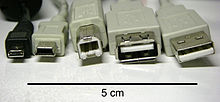
\includegraphics[keepaspectratio,width=0.5\paperwidth]{USB_types_2.jpg}
	\end{center}
	\caption{USB连接器类型}
	从左到右分别为:非USB(私有),mini-B plug, B plug, A receptacle, A plug。
	\label{fig:USBconnectors}
\end{figure}

\begin{figure}[ht]
	\begin{center}
		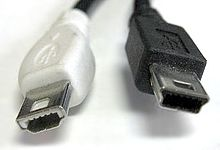
\includegraphics[keepaspectratio,width=0.5\paperwidth]{Mini_usb_AB.jpg}
	\end{center}
	\caption{USB mini连接器类型}
	从左到右分别为:mini-A plug,mini-B plug。
	\label{fig:USBconnectors}
\end{figure}

USB可以连接的外设有鼠标、键盘、游戏手柄、游戏杆、扫描仪、数码相机、打印机、硬盘和网络部件。对数码相机这样的多媒体外设USB已经是缺省接口;由于大大简化了与计算机的连接,USB也逐步取代并行接口成为打印机的主流连接方式。2004年已经有超过1亿台USB设备;到2007年时,高清晰度数字视频外设是仅有的USB未能染指的外设类别,因为他需要更高的传输速率。

现USB标准中,统一为USB 3.0,理论可以向下兼容。一般产商同时提供USB 3(以蓝色特别标示)与USB 2接口,不提供向下兼容USB 2的USB 3接口。

USB实装论坛(USB Implementers Forum,USB-IF)负责USB标准制订,其成员包括:苹果电脑、惠普、NEC、微软和英特尔。

2001年底,USB-IF公布了USB 2.0规范,增加更高的数据传输速率480 Mbit/s(现在称作Hi-Speed)。与之前的USB 0.9、USB 1.0和USB 1.1一样,该规范完全向后兼容。随后,USB-IF公布了USB On-The-Go(USB OTG,当前版本:1.0a)作为USB 2.0规范的补充标准,使其能够用于在便携设备之间直接交换数据。

2007年1月4日,USB-IF颁布了Micro-USB的插头标准。该标准将在许多新型智能手机和PDA上替代Mini-USB。Micro-USB插头的插拔寿命为10,000次,比Mini-USB插头高度减半,宽度相差无几。OMTP组织最近宣布,Micro-USB将成为移动设备数据和电源的标准接口。

USB 3.0于2008年11月释出。USB 3.0支持全双工,比USB 2.0多了数个触点,并采用发送列表区段来进行数据发包。USB 3.0暂定的供电标准为900mA,且支持光纤传输,设计“Super Speed”传输速度为5Gbit/s,若采用光纤则可达到25Gbit/s。USB 3.0的设计兼容USB 2.0与USB 1.1版本,并采用了三级多层电源管理技术,可以为不同设备提供不同的电源管理方案。



\subsection{USB2.0}
\subsection{USB3.0}























